\section{Teststation Output}

\subsection{Pedstal and Noise}
The pedestal noise can be performed in peak or deconvolution mode and with the inverter on or off.
In practice the only test that was relevant for production was deconvolution mode with the inverter on.
This is the standard running mode of the APV for LHC operation.
The output consists of a text file with two columns: the Pedestal values and the corresponding noise, both in ADC counts.
The columns have either 4 x 128 or 6 x 128 entries depending of the number of APVs on the hybrid.
An example for a hybrid with 6 APVs is given in \ref{fig:ped_noise_example}
\begin{figure}[h]
  \begin{center}
    \resizebox{\textwidth}{!}{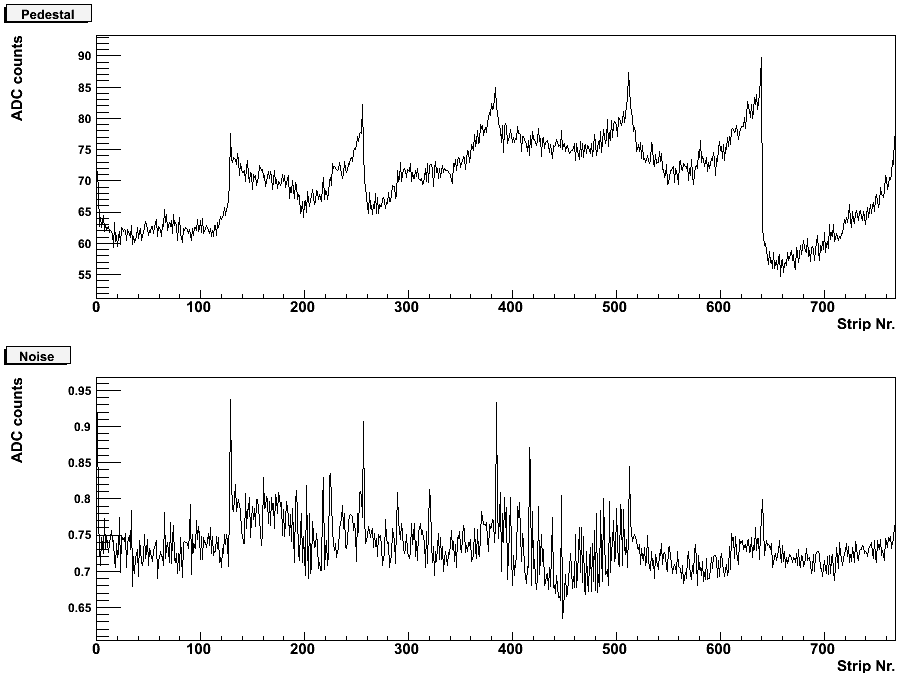
\includegraphics{fig/ped_noise_example.png}}
    \caption{Example for Pedestal and Noise measurement of a hybrid with 6 APVs}
    \label{fig:ped_noise_example}
  \end{center}
\end{figure}


\subsection{Hybrid grading}
An upper and a lower cut are applied on the measured noise values, and channels outside these cuts are considered bad.
The lower noise cut was fixed at 0.6 ADC channels, the upper one at 1.3 ADC channels.
The channel numbers that are found with shorts or opens are stored in text files and displayed at the end of the test as well as the the channels failing the noise cuts.
After all test are finished, the results are automatically analised and the hybrid is graded A, B or 'bad'.
If any test fails to complete, be it in the initialisation or data taking phase, the hybrid is graded as 'bad'.
If all tests finish, the grading is done as follows:
\begin{itemize}
\item[Grade A:] No shorts, less than 4 channels which are open or fail nois cuts
\item[Grade B:] No shorts, between 4 and 6 channels which are open or fail noise cuts
\item[Bad:] Any short or more than 6 channels which are open or fail the noise cuts
\end{itemize}

\subsection{DCU and PLL issues}
If a PLL fails to lock in at low temperatures and needs the initialization procedure described in \ref{}, a corresponding comment is included in the test summary.
For calibration purposes on a fraction of hybrids the temperature below the ceramic was measured as well as the DCU ADC values for channels 0, 4 and 7. These channels measure the temperature inside the DCU, onf a thermistor mounted on the hybrid and \fixme. The values are saved and can be used to intercalibrate the temperature probes on the hybrids.

\subsection{Database feeding}
The hybrid plus PA quality control tests were initially foreseen to be entirely performed at CERN;
While the entire test data have been locally stored, the relevant production and quality control summaries have been sent to the SQL based central tracker database. For this reason the result files are parsed by an XML generator which creates a database compliant XML file. The table TESTWITHPA\_1\_HYB\_ was implemented for the needs of the hybrid test station.

The table TESTWITHPA\_1\_HYB\_ contains the following fields:


Examples of the CERN teststation performances and capabilities are given below; all results refers to hybrid+pa tested at CERN.

A comprehensive review of all hybrids plus PA assembly quality control  performed either at CERN and in the US labs is in preparation.

